\documentclass[a4paper, 11pt, oneside]{article}

\usepackage[utf8]{inputenc}
\usepackage[T1]{fontenc}
\usepackage[english]{babel}
\usepackage{array}
\usepackage{shortvrb}
\usepackage{listings}
\usepackage[fleqn]{amsmath}
\usepackage{amsfonts}
\usepackage{fullpage}
\usepackage{enumerate}
\usepackage{enumitem}
\usepackage{graphicx}
\usepackage{alltt}
\usepackage{indentfirst}
\usepackage{eurosym}
\usepackage{listings}
\usepackage{titlesec, blindtext, color}
\usepackage{float}
\usepackage[nameinlink,noabbrev]{cleveref}
\usepackage{caption}
\usepackage{subcaption}

\usepackage{titling}
\renewcommand\maketitlehooka{\null\mbox{}\vfill}
\renewcommand\maketitlehookd{\vfill\null}

\newcommand{\ClassName}{INFO-0027: Programming Techniques}
\newcommand{\ProjectName}{Project 1: Report}
\newcommand{\AcademicYear}{2020 - 2021}

%%%% Page de garde %%%%

\title{\ClassName\\\vspace*{0.8cm}\ProjectName\vspace{0.8cm}}
\author{Goffart Maxime \\180521 \and Joris Olivier \\ 182113}
\date{\vspace{1cm}Academic year \AcademicYear}

\begin{document}

%%% Page de garde %%%
\begin{titlingpage}
{\let\newpage\relax\maketitle}
\end{titlingpage}

%%%%%%%%%%%%%%%%%%%%%%%%%%%%%%%%%%%%%%%%%%%%%%
\section{Introduction}
\paragraph{}Our implementations rely on 2 different data structures. The first implementation uses a hash table with chaining to solve the potential collisions. The second implementation uses a ternary search trie.
\paragraph{}We decided to perform our performance study by testing our implementations with an increasing number of addresses in order to be able to analyse the differences between the implementations on graphics. For each number of addresses we were considering, we did 1000 different creations of the MAGIC A.D.T. and measured the mean time passed in the \texttt{MAGICindex}\footnote{We called MAGICindex on each address that was randomly generated.} and \texttt{MAGICreset} functions, and the mean amount of allocated memory. 
\paragraph{}For each of the 1000 tests, we used randomly generated 4 bytes addresses. The same batch of randomly generated addresses was used for the two different implementations.

\section{Time performance}
\paragraph{}In this section, we will compare the time spent in the \texttt{MAGICindex} and \texttt{MAGICreset} functions depending on the implementation being used. We will also compare the total time spent.

\subsection{MAGICindex function}
\paragraph{}For the \texttt{MAGICindex} function, we obtained the following chart:
\begin{figure}[H]
  \centering
  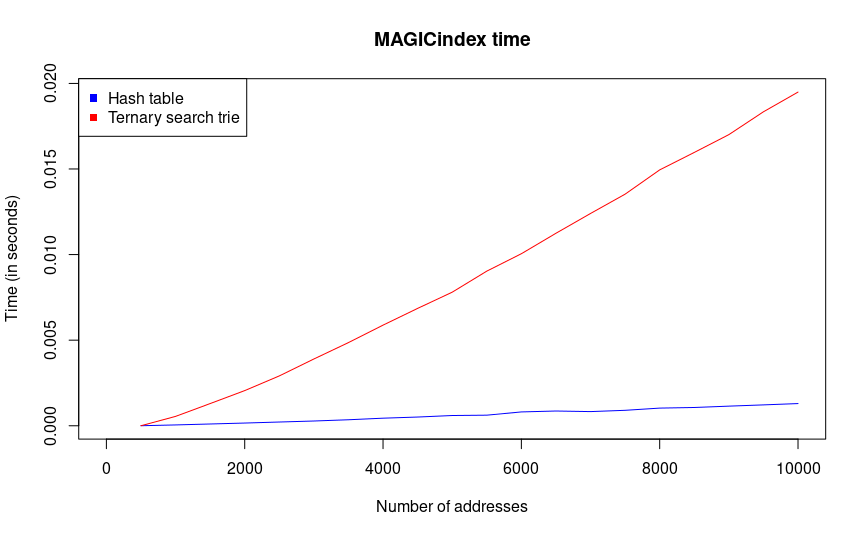
\includegraphics[scale=.5]{plots/index.png}
  \captionof{figure}{Mean time passed in the \texttt{MAGICindex} function depending on the number of addresses}
\end{figure}
We can easily observe that the implementation using a hash table is faster than the one using a ternary search trie. This is not an unexpected result because a search in a hash table has an average complexity of $\mathcal{O}(1)$ while a search inside a TST has an average complexity of $\mathcal{O}(log(n))$ where $n$ is the number of elements being stored.

\subsection{MAGICreset function}
\paragraph{}For the \texttt{MAGICreset} function, we obtained the following chart:
\begin{figure}[H]
  \centering
  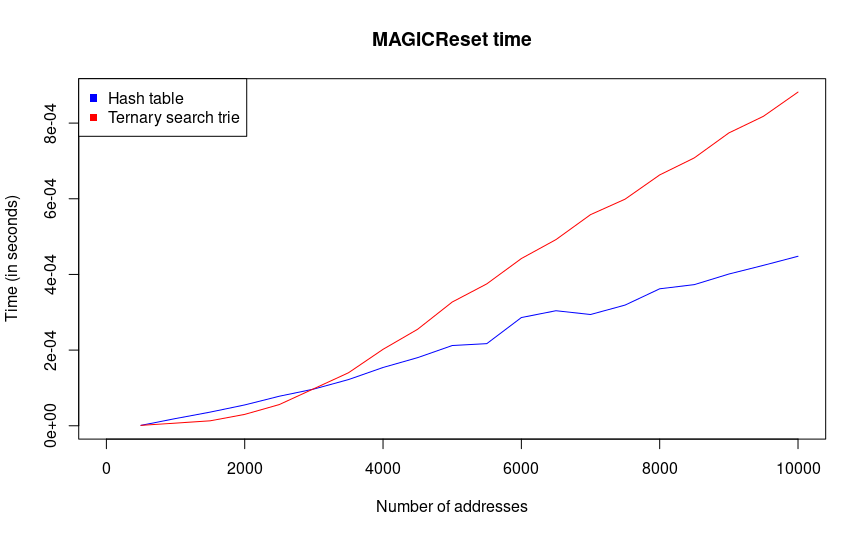
\includegraphics[scale=.5]{plots/reset.png}
  \captionof{figure}{Mean time passed in the \texttt{MAGICreset} function depending on the number of addresses}
\end{figure}
We can observe that the TST implementation is faster when we store less than $\pm$ 3000 addresses. After that, the hash table implementation is faster. The slight advantage in time procured by the TST implementation for less than $\pm$ 3000 addresses, can be considered has insignificant due to how small the time differences are (a few tenth of a millisecond). In general, we can conclude that both implementations of the \texttt{MAGICreset} function are fast to execute because we are talking in tenths of a millisecond.

\subsection{Total time}
\paragraph{}For the total time spent, we obtained the following chart:
\begin{figure}[H]
  \centering
  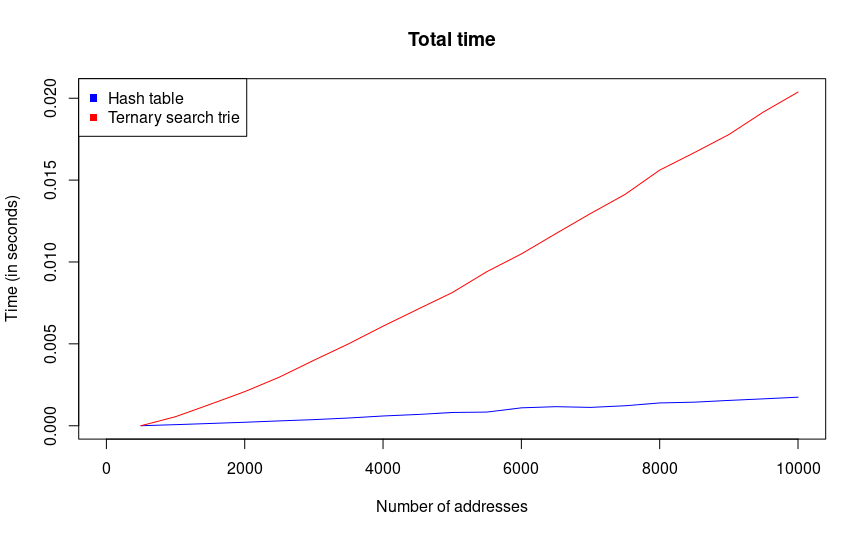
\includegraphics[scale=.5]{plots/general.png}
  \captionof{figure}{Mean time passed in the A.D.T. functions depending on the number of addresses}
\end{figure}
Since the time spent in the \texttt{MAGICindex} and \texttt{MAGICreset} functions was smaller for the implementation using a hash table, it is logical that the total time is smaller for the implementation using a hash table.

\section{Memory perfomance}
\paragraph{}For the amount of memory being allocated, we obtained the following chart:
\begin{figure}[H]
  \centering
  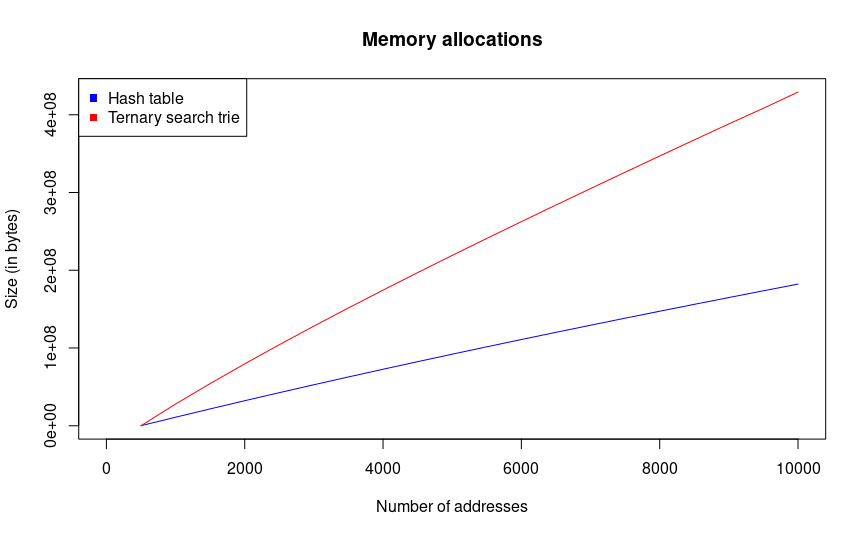
\includegraphics[scale=.5]{plots/mem.png}
  \captionof{figure}{Mean amount of memory allocated depending on the number of addresses}
\end{figure}
We can observe that the implementation using a hash table uses less memory than the one using a TST. This can be explained by the fact that each node in the TST stores 3 pointers, one digit, and an Item. While the hash table uses only an array of linked list (the linked list being used to solve the collisions by chaining). If there is no collision at all, it uses a bit more memory than an array of pointer because we need to store the index in the auxiliary array.

\section{Conclusion}
\paragraph{}In conclusion, we observed that our first implementation, which uses a hash table, has better performances than our second one, which uses a ternary search trie, in terms of time and memory.

\end{document}
